\documentclass[portrait]{Hylangtechposter}
\graphicspath{{./figures/},{./Plots/media/images/}} % Location of the graphics files


\begin{document}


\printheader

\begin{center}
%% TITLE
\textbf{\bf\veryHuge\color{Purple} Cálculo de flujo alrededor de un perfil alar mediante la técnica de mapeo conforme \\[0.5cm]}

%% AUTHORS

\huge     Daniel Carrete $^1$  ~
    Edwin Pérez$^2$  ~ 
    Jesús Camacho$^3$~ 
  
\Large    \texttt{ $^1$a348564@uach.mx} \qquad \texttt{$^2$a348643@uach.mx} \qquad \texttt{$^3$a348674@uach.mx} 
 

 \end{center}


%%%% If you have an abstract:  uncomment %%%%
%%%%
% \color{Navy}
% \begin{abstract}


  
% \end{abstract}

\vspace{0.3cm}

% \large \Large \LARGE \huge \Huge \veryHuge \VeryHuge \VERYHuge

 \Large

\begin{multicols}{2} % begin two columns

  \color{black}
  
\section*{Introducción}
\noindent La técnica de mapeo conforme en variable compleja es una herramienta matemática
que permite transformar regiones del plano complejo en otras regiones de manera que
se preserven los ángulos y se conserven algunas propiedades geométricas. \\
Lo que buscamos es visualizar  cómo es un fluido en un perfil alar,  
ya conociendo con anterioridad el comportamiento en una región diferente, y adaptándola por medio de una transformación.
% \color{DarkSlateGray} % DarkSlateGray color for the rest of the content
\section*{Marco Teórico}
\noindent Empezaremos con uno de los resultados de flujo importantes obtenidos mediante el mapeo conforme, que son las soluciones del flujo de una familia de formas aerodinámicas, conocidas como perfiles de Joukowski, que son el resultado de la transformada de Joukowski, la cual tenemos a continuación:
\begin{equation}
    \zeta = \eta + \frac{a^2}{\eta},
\end{equation}
donde ``a'' es una constante que determina la fuerza y la forma de la transformación.
\begin{center}\vspace{0.5cm}
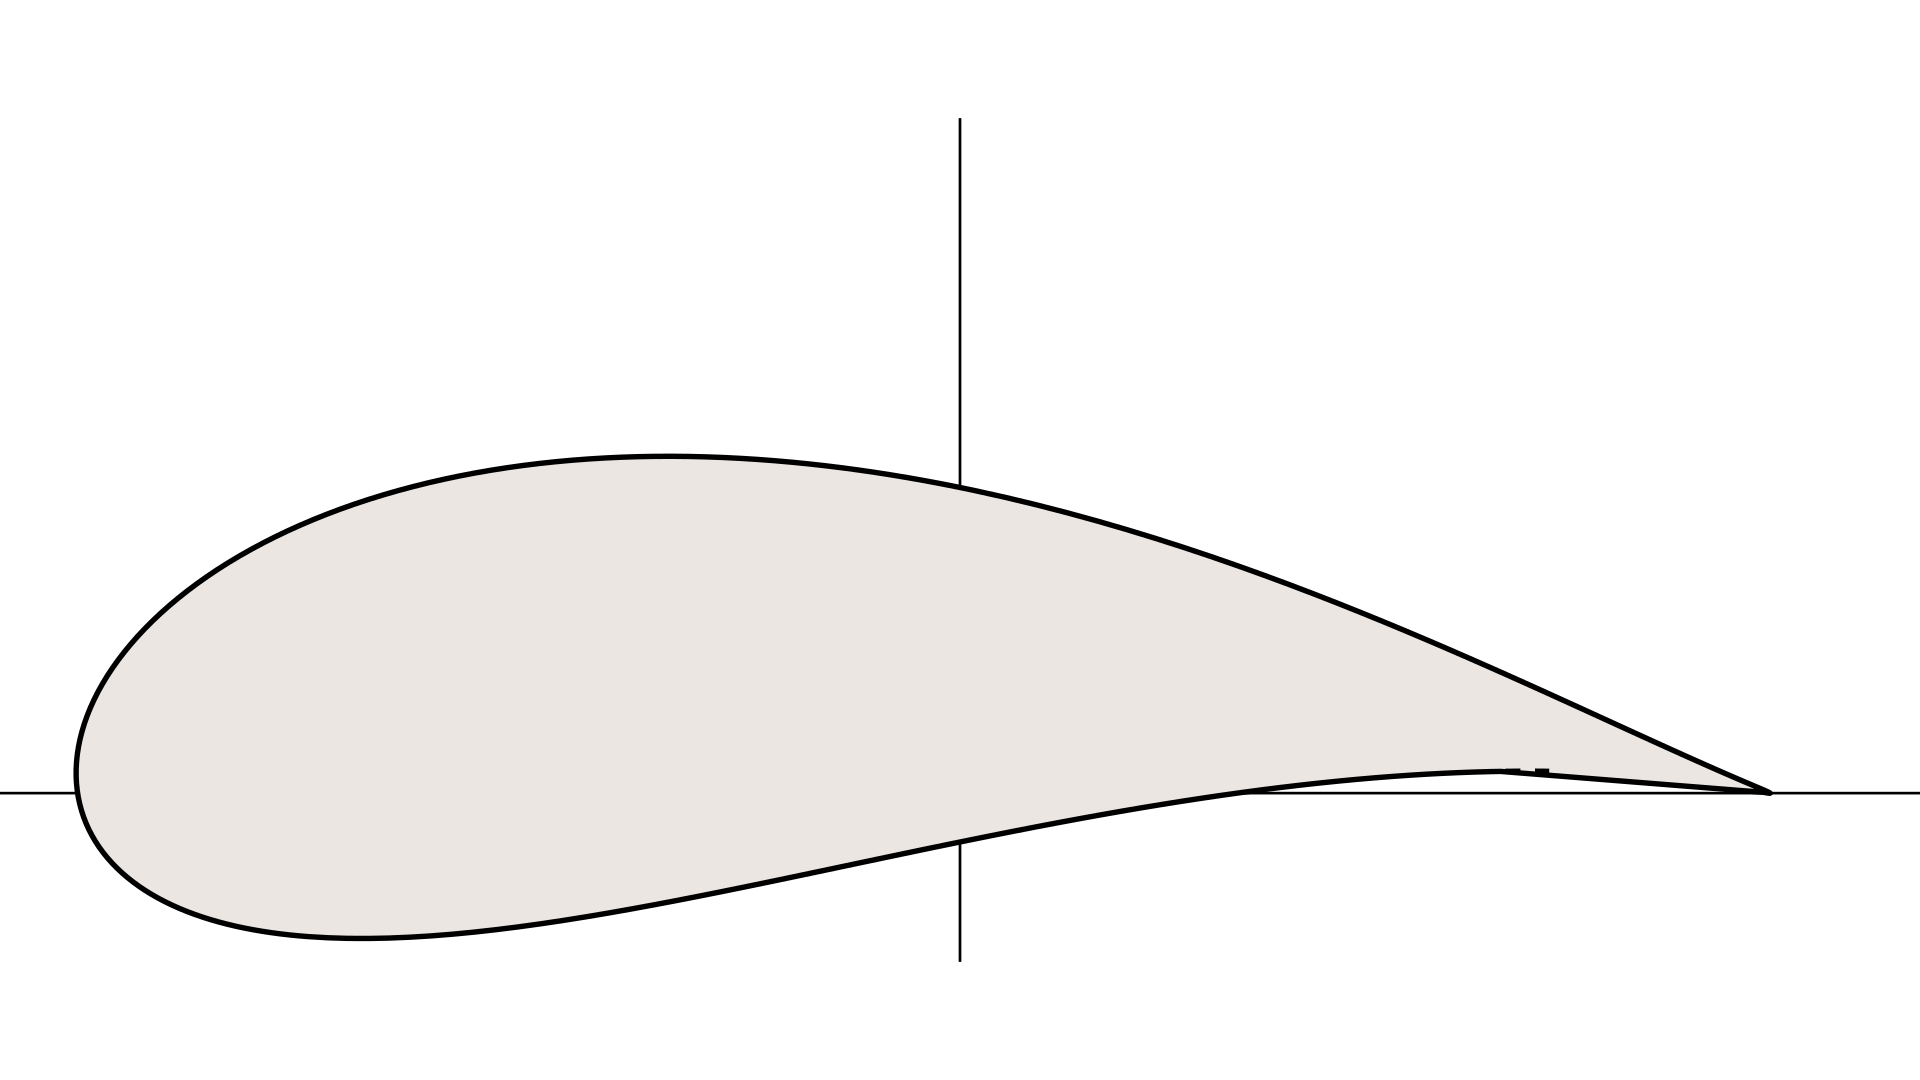
\includegraphics[scale=0.3]{Airfoil_ManimCE_v0.17.1.png}
\captionof{figure} {Perfil alar de Joukowski.}
\end{center}\vspace{0.5cm}
De manera que podemos encontrar primero la solución en el flujo que pasa alrededor
de un perfil circular para después hacer uso del mapeo conforme para
transformar el círculo en una forma aerodinámica conservando la solución.
\begin{center}\vspace{0.5cm}
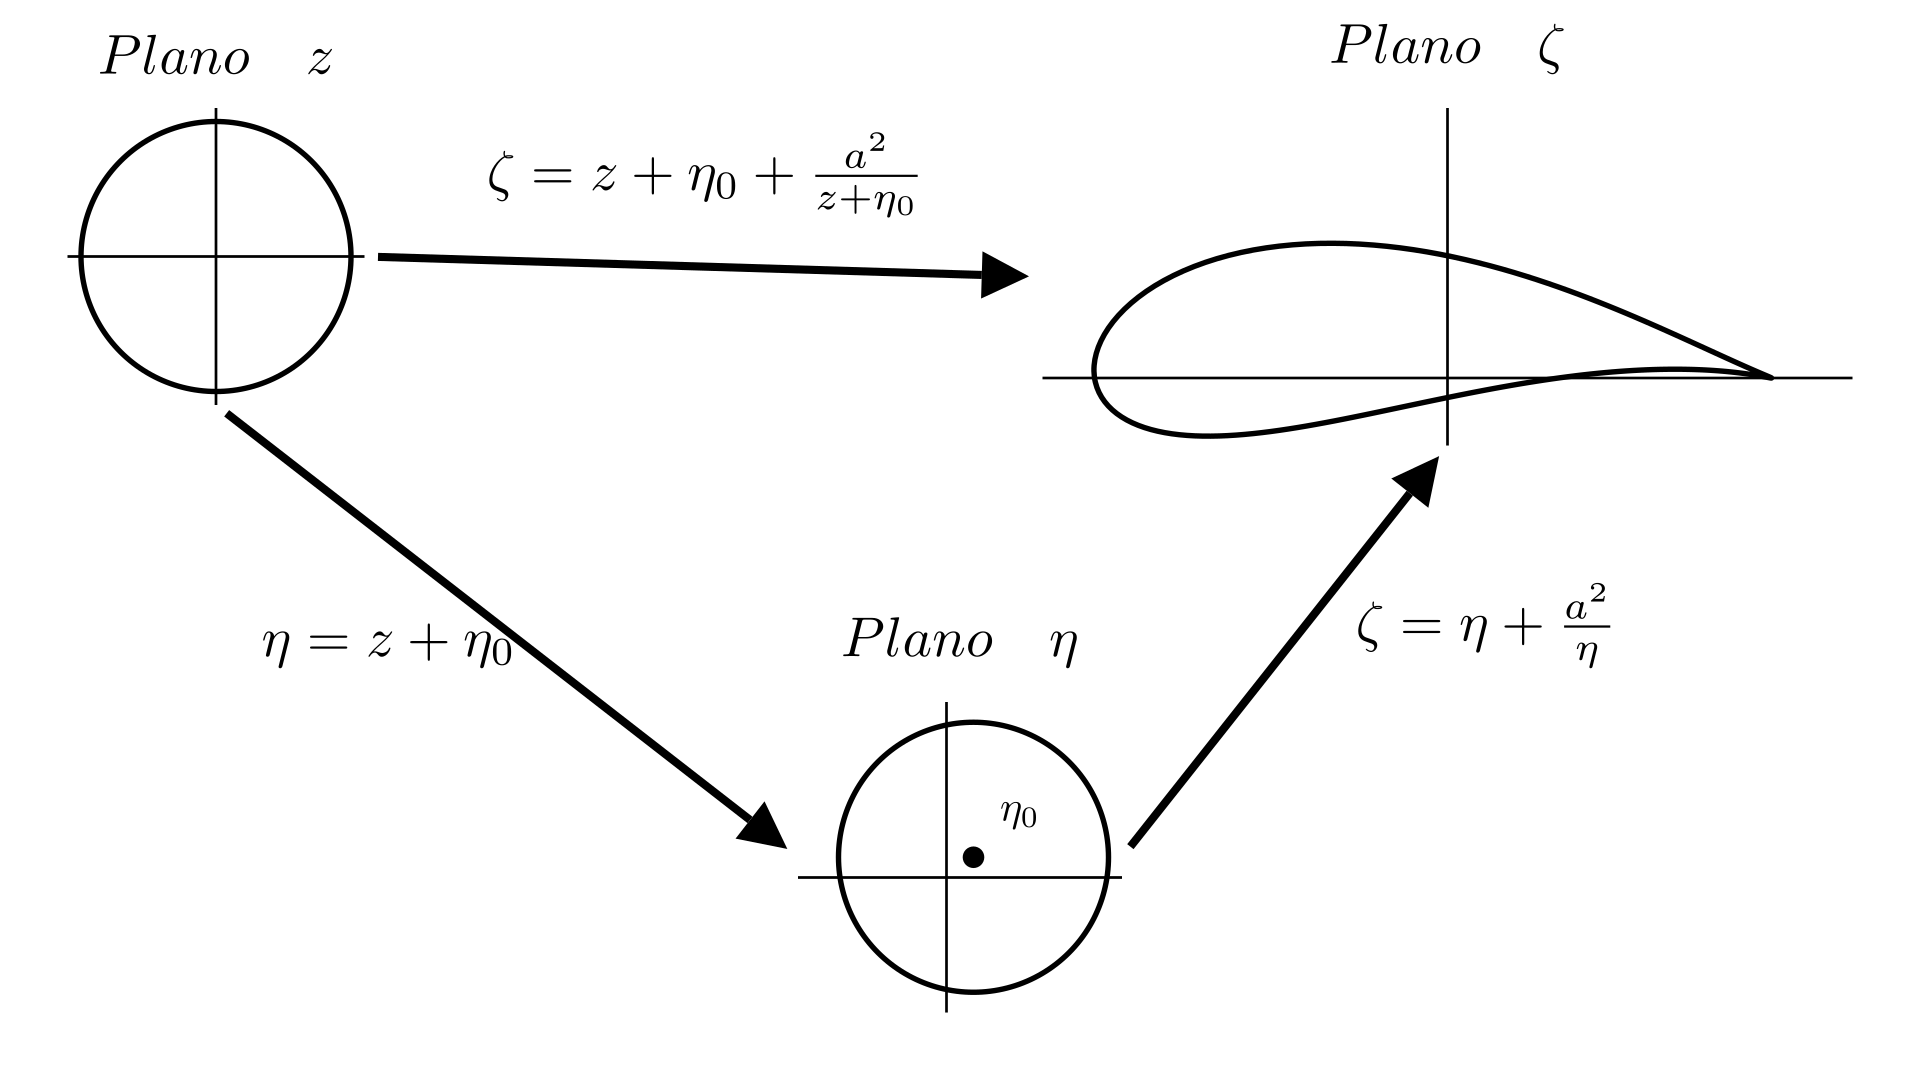
\includegraphics[scale=0.3]{JoukouskiTransform_ManimCE_v0.17.1.png}
\captionof{figure} {Transformada que se realiza para mapear un círculo unitario del
plano z al perfil alar. }
\end{center}\vspace{0.5cm}
Consideramos que el movimiento del fluido está dado por un campo vectorial de velocidades $\vec{V}(x,y,z)$, además consideremos que el fluido es irrotacional, es decir, que se cumple $\vec{\nabla} \times \vec{V}=0 $ lo que implica que debe de existir una función de potencial de velocidad tal que $\vec{\nabla}\varphi = \vec{V}$. Lo cual nos da paso a la ecuación de continuidad para dinámica de fluidos:
	\begin{equation}
		\frac{\partial \rho}{\partial t} + \vec{\nabla} \cdotp (\rho \vec{V}) =0.		
	\end{equation}
 Si el fluido no varía en densidad $\rho$ es decir que $\frac{\partial \rho}{\partial t} =0 $, implica $\vec{\nabla} \cdotp (\rho \vec{V}) = 0 \longrightarrow \vec{\nabla} \cdotp (\vec{V}) =0 $, o en términos de la función potencial,
	\begin{equation}
		\vec{\nabla} \cdotp (\vec{\nabla}\varphi) = \nabla^2 \varphi =0.
	\end{equation}	 

 \noindent La teoría de potencial en su mayor parte es el estudio de funciones armónicas, o en otras palabra funciones que satisfagan la ecuación de Laplace.\\
 Si consideramos que el flujo no tiene componente en $z$ podemos asumir que el potencial de velocidad será bidimensional  $\varphi(x,y)$, tal que $\vec{\nabla}^2 \varphi =0 $ en algún dominio $D$ del plano, y tomemos a $\varphi$ como la parte real de una función analítica compleja
	\begin{equation}
		F(z)=\varphi (x,y)	+ i \psi(x,y).
	\end{equation}
	$F(z)$ se llama el potencial complejo, donde $\psi$ es llamada  función de flujo que al igualarla a una constante $c_n$, representa las líneas de flujo del fluido.
Si una frontera sólida es colocada en el fluido, implica que esta representa una línea de flujo, por lo que el problema se reduce  a buscar una función de flujo $\psi$ para esa frontera que pueda ser representada como $\psi=c_0$, una vez que la función pueda ser encontrada la velocidad puede ser calculada con la ecuaciones de Cauchy-Riemann
	\begin{equation}
		\begin{split}
			v_x &= \frac{\partial \varphi}{\partial x} = \frac{\partial \psi}{\partial y }, \\
			v_y &= \frac{\partial \varphi}{\partial y} =- \frac{\partial \psi}{\partial x }. \\
		\end{split}
	\end{equation}

 
\section*{Desarrollo}
\noindent Considere ahora un flujo uniforme con velocidad $U_0$ en la dirección $x$, con un potencial complejo $F(z)= U_0 z$, si se coloca un obstáculo circular en $|z| =R$ provocará que el fluido sea desviado. \\
	\noindent Para intentar resolver la función de potencial que tendrá el círculo usaremos un resultado encontrado por el matemático inglés L.M. Milne-Thompson.
		
			\begin{equation}
				W(z) = F(z) + \overline{F \left( \frac{R^2}{\overline{z} }\right)} .
				\label{Teorema_del_circulo}
			\end{equation}
			Donde la barra denota el complejo conjugado, tiene las mismas singularidades que $F(z)$ en $|z|>R $, y el círculo denotado por $|z|= R $ es una línea de flujo.
		
  \noindent Podemos darnos cuenta de que el potencial $F(z)= U_0 z$ satisface lo anterior, por lo que podemos obtener el potencial complejo  del flujo alrededor de un círculo sustituyendo $F(z)= U_0 z$ en (\ref{Teorema_del_circulo}) 

		\begin{equation}
			W(z) = U_0 z + \frac{\overline{U_0 R^2} }{\overline{z} } = U_0 z +\frac{U_0 R^2}{z} ,
			\label{PotencialCirculo}
		\end{equation}

		\noindent y la función de flujo es la parte compleja de $W$ 
		\begin{equation*}
			Im[W(z)]=\psi =  U_0 y \left( 1- \frac{R^2}{x^2 + y^2}\right).
			\label{Potencial}
		\end{equation*}
			\begin{center}\vspace{0.5cm}
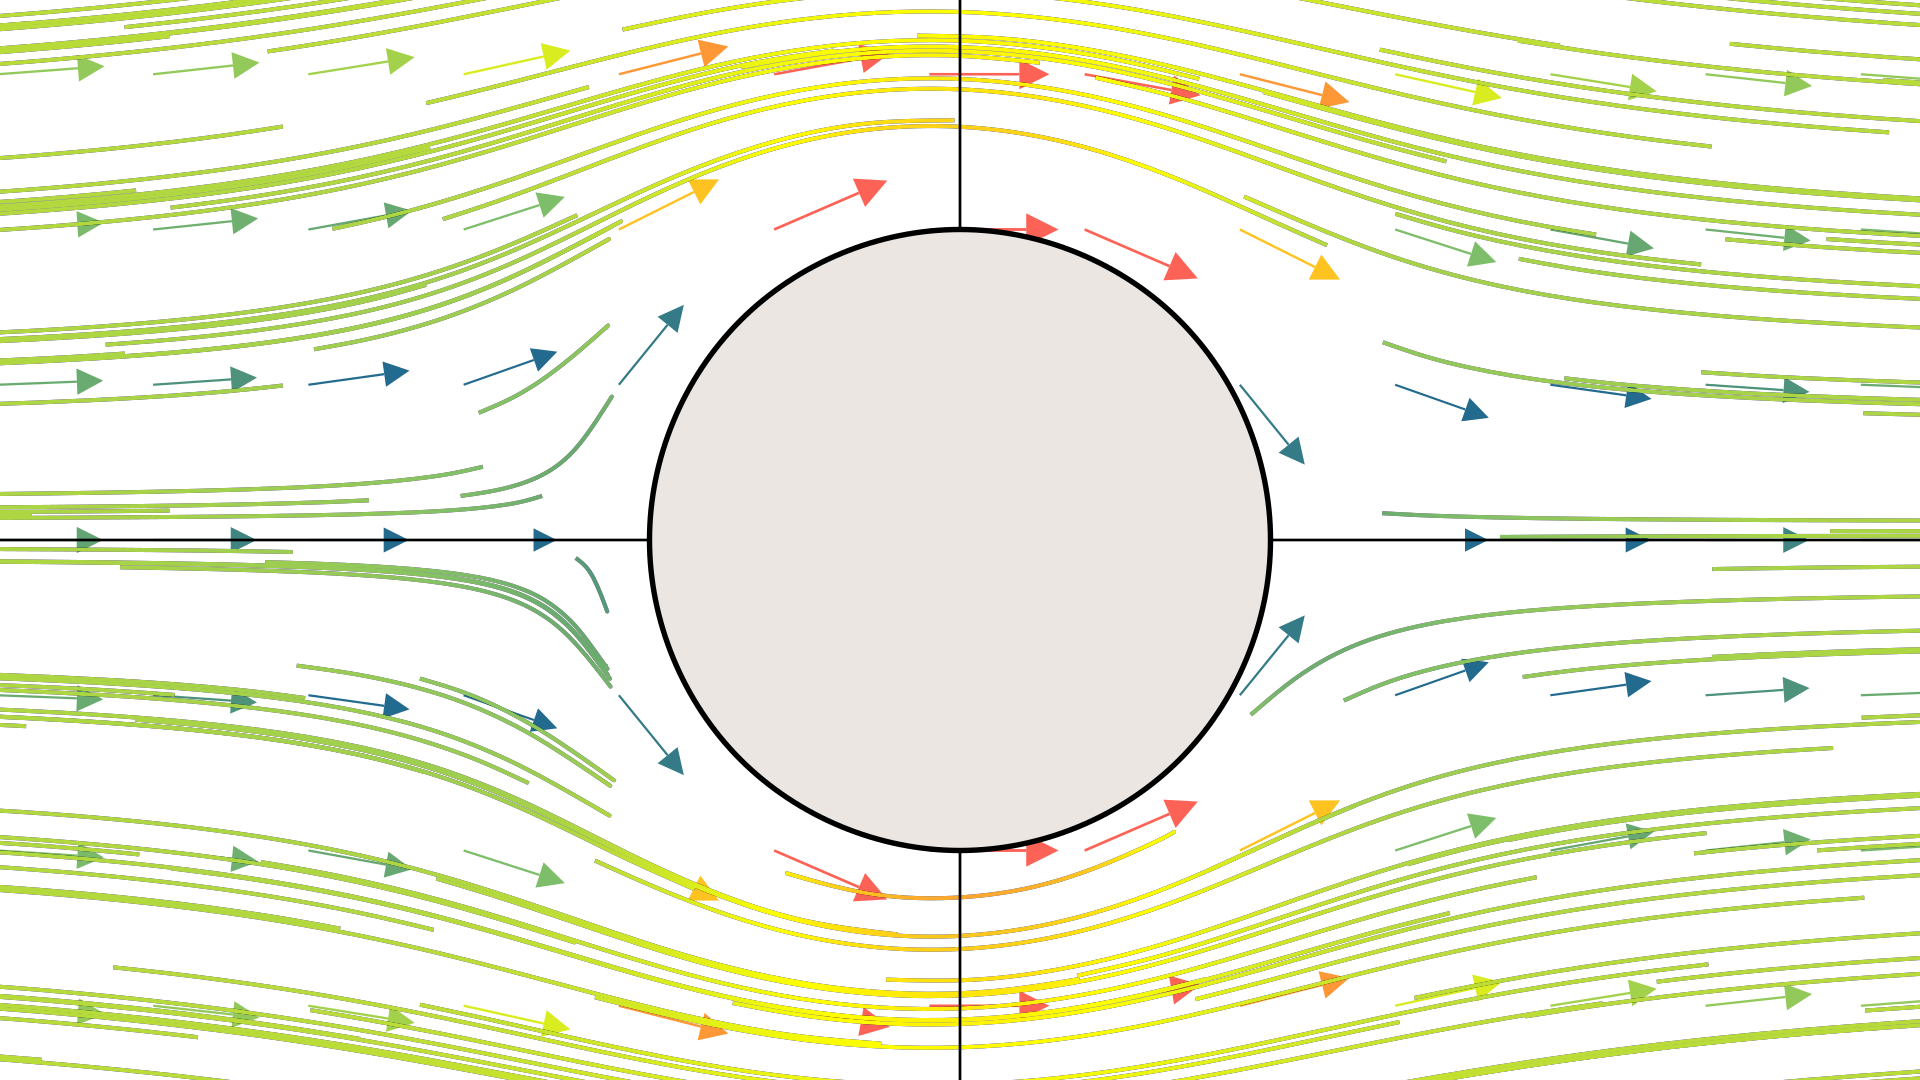
\includegraphics[scale=0.25]{FlowAroundCircle_ManimCE_v0.17.1}
\captionof{figure} {Campo de velocidades de un fluido con un obstáculo circular.}
\end{center}\vspace{0.5cm}
Si agregamos un vórtice al potencial definido en (\ref{PotencialCirculo}) se obtiene el potencial de flujo con circulación
			\begin{equation}
				W(z) = U_0z + \frac{ U_0R^2}{z} + \frac{i \Gamma}{2 \pi}\log (z),
			\end{equation}
			donde  $\Gamma$ es la circulación hallada empleando la condición de Kutta (una condición de límite viscoso basada en la observación física utilizada con un modelo teórico no viscoso).

			
			Después de hacer la transformación del círculo unitario en el plano $z$ al plano $\eta$, y en este caso la función de flujo es 
			\begin{equation*}
				\psi = \frac{\Gamma \log{\left(\sqrt{x^{2} + y^{2}} \right)}}{2 \pi} - \frac{R^{2} u_{0} y}{x^{2} + y^{2}} + u_{0} y.
			\end{equation*}
\begin{center}\vspace{0.5cm}
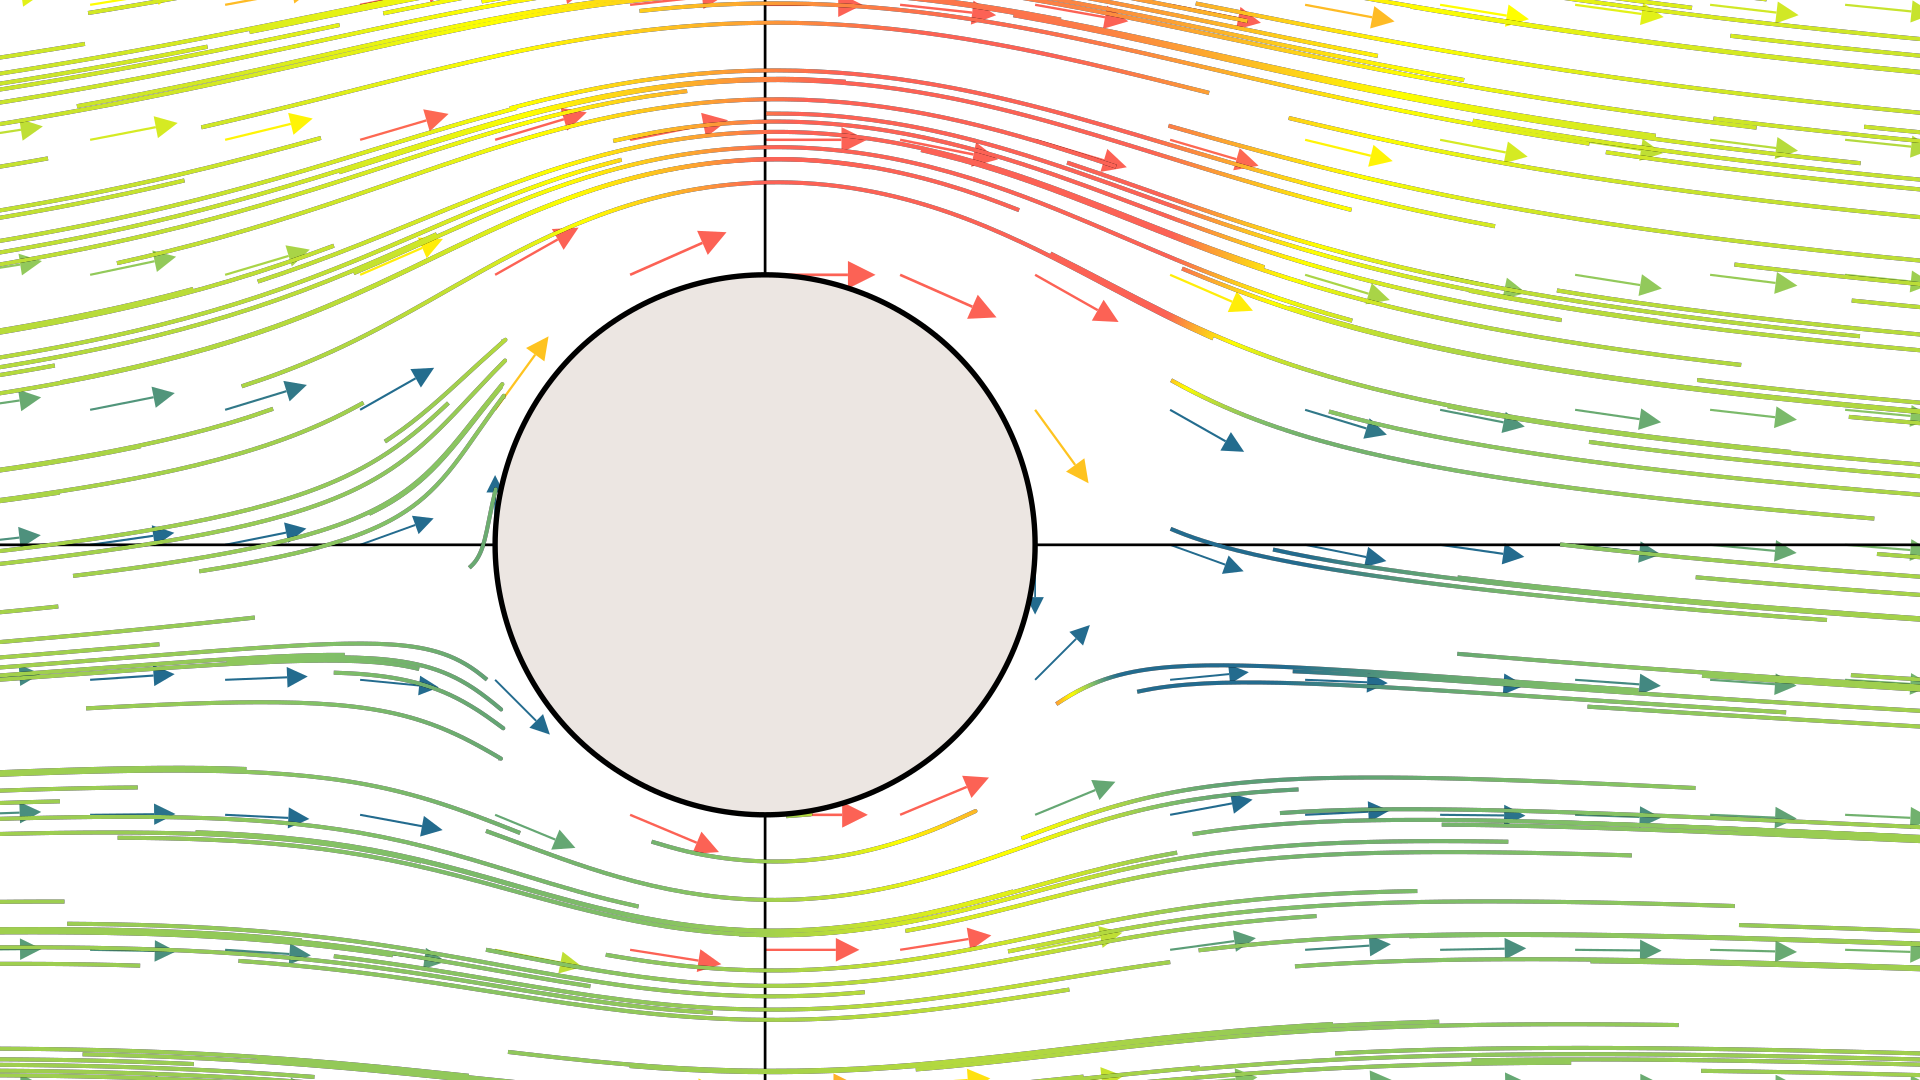
\includegraphics[scale=0.25]{StreamLinesCircleCirculation_ManimCE_v0.17.1}
\captionof{figure} {Velocidades en un fluido con circulación (puede apreciarse como la parte
superior del círculo tiene una velocidad mayor a la parte inferior de este).}
\end{center}\vspace{0.5cm}

\noindent Ahora que se conoce el potencial complejo $W(z)$ que está asociado al $plano \: z$ es posible mapear el potencial de cada punto en el $plano \: z$ hacia el $plano \: \zeta$; nuestros requerimientos nos exigen que tengamos una función de potencial complejo que llamaremos $\Xi(\zeta)$ que representa el potencial complejo en el plano $\zeta$ en función de cada punto en este mismo.
			
			De manera similar a como se hizo la composición de funciones en la figura $2$ se obtiene una función $Z(\zeta)$, tal que podemos evaluar en el potencial asociado al plano $z$ y obtener el potencial en el plano $\zeta$,

			\begin{equation*}
				\Xi(\zeta)= W(Z(\zeta))	= \Phi +i \Psi,			
			\end{equation*}
			y la función inversa es
			\begin{equation*}
				Z(\zeta)= \frac{1}{2}\left(\zeta \pm  \sqrt{\zeta^2 -4R^2} \right) - \eta_0 . 
			\end{equation*}
			Haciendo la evaluación $W(Z(\zeta))$ para obtener el potencial del plano $\zeta$ se obtiene
			
			\begin{equation}
				\begin{split}
					W(Z(\zeta)) = \Xi(\zeta) =& U_0 \left( \frac{1}{2}\left(\zeta \pm  \sqrt{\zeta^2 -4R^2} \right) - \eta_0\right) + \frac{ U_0R^2}{\frac{1}{2}\left(\zeta \pm  \sqrt{\zeta^2 -4R^2} \right) - \eta_0}\\ 
					&+ \frac{i \Gamma}{2 \pi}\log \left(\frac{1}{2}\left(\zeta \pm  \sqrt{\zeta^2 -4R^2} \right) - \eta_0\right),\\
				\end{split}	
			\end{equation}
			cuya función de flujo $\Psi $ es,
			\begin{equation*}
				\Psi=Im[\Xi(\zeta)] .
			\end{equation*}
			
			\noindent Por motivos de simplicidad no mostraremos cuanto vale $v_x$ y $v_y$ pero se sobrentiende que es
			\begin{equation*}
				\begin{split}
					v_x &= \frac{\partial \Psi }{\partial y},\\
					v_y &= -\frac{\partial \Psi }{\partial x},
				\end{split}
			\end{equation*}
			y aquí la representación del flujo en el perfil alar original.

\begin{center}\vspace{0.5cm}
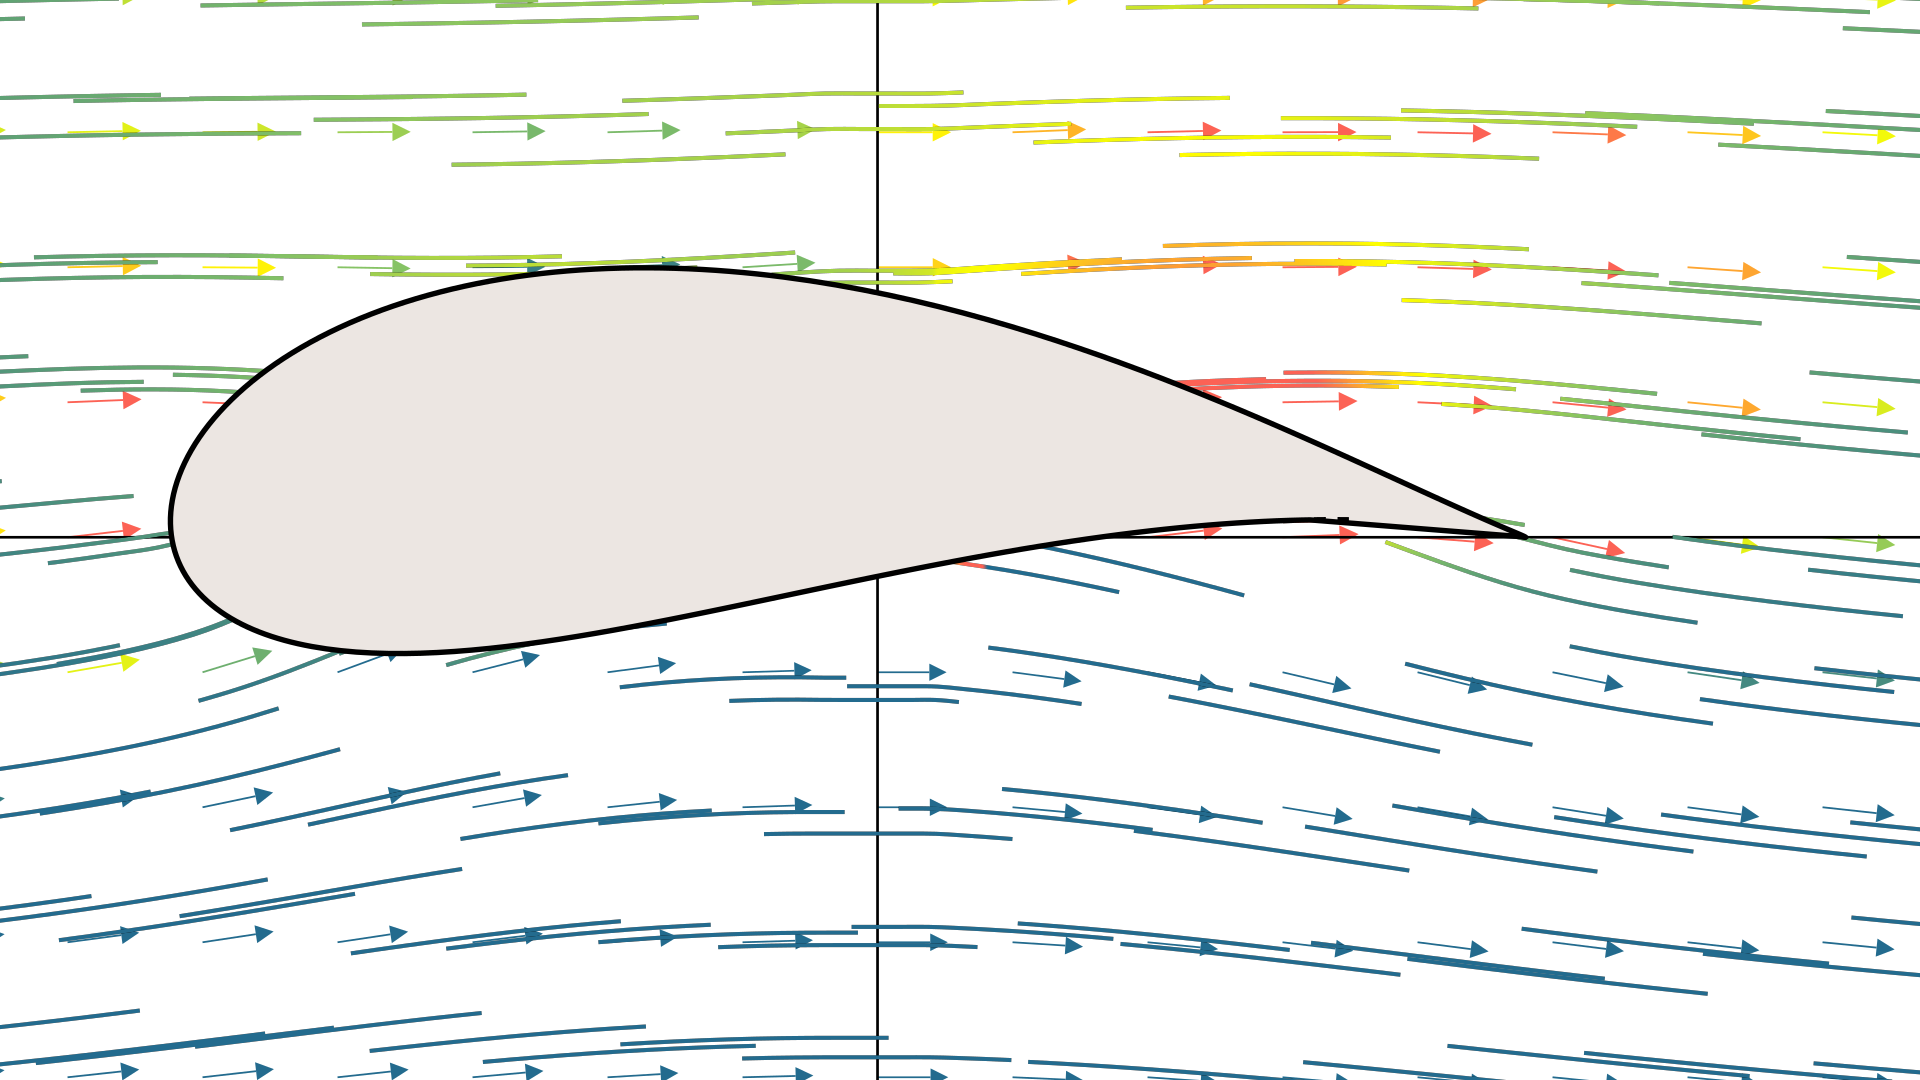
\includegraphics[scale=0.25]{StreamLinesAirfoil_ManimCE_v0.17.1.png}
\captionof{figure} {Campo de velocidades de un fluido con un obstáculo alar.}
\end{center}\vspace{0.5cm}
\section*{Conclusión }

\noindent En resumen, el uso del mapeo conforme en el cálculo del flujo alrededor de un perfil alar proporciona una herramienta poderosa y versátil para analizar y diseñar perfiles aerodinámicos. Esta técnica simplifica el análisis matemático, mejora la precisión de las soluciones y facilita la comprensión visual del flujo, lo que contribuye al desarrollo de perfiles más eficientes y aerodinámicamente óptimos.


\begin{thebibliography}{X}
\large \bibitem{Baz}  \textsc{R. A. Silverman, Complex analysis with applications. New York: Dover Publications, (1984), págs. 228-238 }
\large \bibitem{Dan} \textsc{ J. W. Dettman, Applied complex variables. Macmillan (N.Y.); Collier-Macmillan, (1965) págs. 229-234} 

\end{thebibliography}

\end{multicols}

\end{document}  